
\chapter{Online {\IterComp}}\label{chap:oic}

This chapter describes the overall architecture for the online {\itercomp} guided by the work-based performance metric.
Section~\ref{sec:metric} defines the work-based performance metric, with a focus on how it enables the comparison between different optimised versions of a program.
Section~\ref{sec:oic-infra} details the infrastrcture necessary for performing online {\itercomp}.

\section{Work-based Performance Metric}\label{sec:metric}

In this section we define the work-based performance (WP) metric proposed for comparing different optimised versions of a program when executing with different inputs.
We define the performance metric as the ratio between the amount of \textit{work}, $\Delta W$, performed during a period of time, $\Delta t$.
\[
   P = \frac{\Delta W}{\Delta t}
\]

%The hypothesis is that, given two optimisations $o_1$ and $o_2$, a program compiled with optimisation $o_2$ would \textit{consistently} perform better than when it is compiled with $o_1$, i.e., $o_1 \tilde{<}_p \, o_2$, if it performs more \textit{work} per unit of time when compiled with $o_2$ instead of $o_1$. 
By measuring the amount of \textit{work} done per unit of time we reduce the impact of input-dependent aspects and focus instead on the efficiency of the optimised program.
For this metric, the main challenge is to precisely define what represents \textit{work}.
As discussed in Section~\ref{sec:related-metrics}, many work metrics have been presented in the literature, such as block frequency and others.
However, for comparing the performance benefits of different compiler optimisations on a program, although block frequency would be able to capture aspects of optimisations that simplify the control-flow graph (CFG), we argue that measuring work only at the basic block resolution would not be enough for capturing the effects of optimisations at the instruction level.
For this reason, we extend the idea of using basic block frequency to measure computational work by also considering the computational cost of each basic block.

%For that purpose, we intend to use profiling techniques to measure the input size and amount of computation performed on the execution path triggered by the input~\cite{ball94,ball96,zaparanuks12,coppa14}.
%In addition to being useful for speeding up {\itercomp} across a large number of different inputs, this metric based on comparing work-based efficiencies could
%potentially be used for applying {\itercomp} \textit{online}.
%However, the overhead for estimating the amount of \textit{work} must be low enough for the performance gains to be beneficial.
To this end, we model the computational work $\Delta W$ as a linear equation based on block frequency information and a cost model of the instruction set.
Formally,
\[
\Delta W = \varepsilon + \sum_{B} w(B)f(B)
\]
where $f(B)$ represents the frequency of basic block $B$ and $w(B)$ represents the computational work of executing $B$.
We define the work of a basic block $B$ as the sum of the cost of its instructions, i.e.,
\[
w(B) = \sum_{i} w_i N_B(i)
\]
where $w_i$ is the cost of instruction $i$ and $N_B(i)$ is the number of occurrences of instruction $i$ in basic block $B$.

In this simplified model, we consider that $w_i$ is constant across all programs and executions, varying only between target architectures.
On the other hand, $N_B(i)$ is a program-dependent static value which is known at compile-time and $f(B)$ is a dynamic value known only at run-time,
since $f(B)$ is both program and execution dependent as the execution frequency of a basic block can change when executing with different inputs.
%However, $N_B(i)$ is program dependent but constant across executions, while $f(B)$ is both program and execution dependent, since $f(B)$ can change when executing with different inputs.
%In other words, $N_B(i)$ is a static value known at compile-time and $f(B)$ is a dynamic value known only at run-time.

%If we define $x_i$ as
%\[
%x_i = \sum_{B\in P} N_B(i)f(B)
%\]
%we can write our definition of work $\Delta W$ as the following linear equation
%\[
%\Delta W = \varepsilon + \sum_{i\in I} w_i x_i
%\]

%\subsection{Linear regression}
%
%\begin{figure}[htb]
%    \centering
%    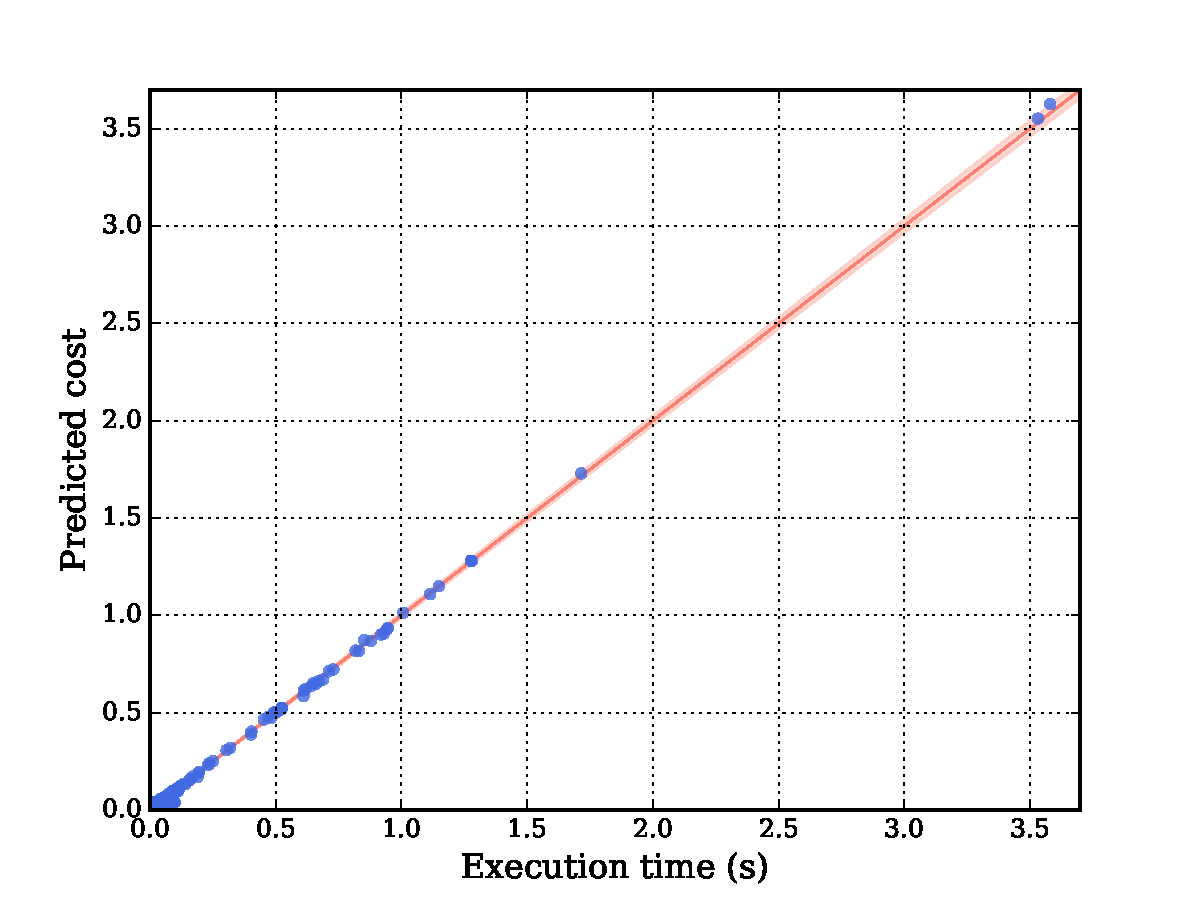
\includegraphics[width=\linewidth]{figs/cost-model.pdf}
%    \caption{Comparison between the naive and optimal instrumentation with no compiler optimisation.} %, i.e., compiled with \textbf{\texttt{-O0}}.}
%    \label{fig:cost-model}
%\end{figure}
%mse 0.000145373168444
%mae 0.00737261168981
%mae* 0.0033892281406
%mape 75.2924320971
%corr (0.99946441743545622, 0.0)

\subsection{Estimating a Cost Model of the Instructions}

Similarly to previous work~\citep{giusto01,powell09,brandolese11}, we derive the cost model of the instruction set by modelling the problem as a multi-variable linear regression, where the \textit{regression coefficients} are the costs of the instructions and the \textit{regressors} are computed as $\sum_B N_B(i)f(B)$ for each instruction.
\begin{equation}\label{eq:linear-work-expression}
\Delta W = \varepsilon + \sum_{i} \left(w_i \sum_{B} N_B(i)f(B)\right)
\end{equation}
By having some empirical data after executing several benchmarks with different inputs, we can fit the linear model with this empirical data in order to obtain estimate costs of the instructions.
In order to fit the linear model, we measure the wall-clock time when executing the training benchmarks described in Section\ref{sec:benchmarks} with their respective 1000 input datasets.
For these measurements, the training benchmarks are compiled without optimisation.
The reason for using no optimisation, as discussed in Section\ref{sec:oic-infra}, is because the amount of work must be only input dependent and consistent between different optimisation sequences.
This aspect is crucial for the work-based performance metric to enable a consistent comparison between different optimisation sequences when executing with distinct inputs.
%it allows to use the estimated cost model for computing a work metric which is independent of optimisations, as we explained in Section~\ref{}.

Our cost model has a total of 52 LLVM instructions\footnote{We do not model all LLVM instructions because some instructions are more common in optimised programs, such as the vector instructions.}.
Every program, in the set of training benchmarks, was compiled twice: once including the necessary instrumentation for the block frequency profiling, which is required for deriving the linear expression defined in Equation~\ref{eq:linear-work-expression};
and a standard compilation without any optimisation or instrumentation.
For each input in the training dataset, the benchmarks were executed once with the instrumented version for collecting the block frequency profiling, and multiple times with the standard compilation just for measuring the wall-clock execution time, until the confidence interval was no larger than 1\% for a 99\% confidence.
After collecting these measurements, this data can be used to estimate the unknown parameters in the linear model.
Because we fit the linear model based on the wall-clock execution time, the derived cost model can be interpreted as an estimate of the execution time when the program is compiled without optimisations.

\begin{figure}[htb]
    \centering
    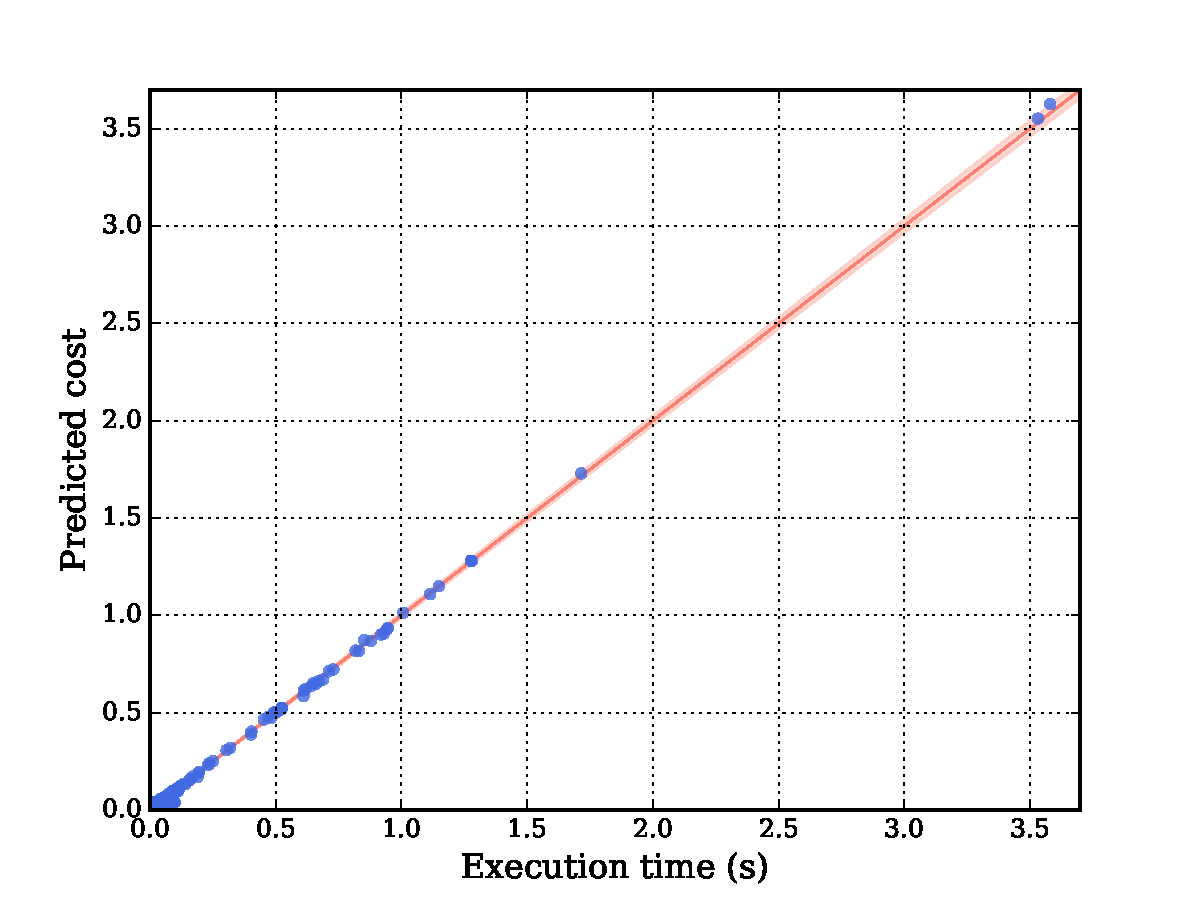
\includegraphics[width=0.9\linewidth]{figs/cost-model.pdf}
    \caption{Linear model fitted from empirical data. The mean absolute error (MAE) for the fitted curve is of 7 milliseconds.}
    \label{fig:cost-model}
\end{figure}

Figure~\ref{fig:cost-model} compare the work metric with the corresponding execution time for some instances of the test benchmarks.
Notice how the fitted model has a higher relative error for the instances with very short execution time, namely those that run for less than one tenth of a second.
The mean absolute error (MAE) for the fitted curve is of 7 milliseconds.

\subsection{Comparison with Instructions Per Cycle} \label{sec:ipc-vs-work-metric}

The IPC metric have been widely used for studying performance benefits of hardware optimisations.
Although previous work have suggested the use of IPC for guiding {\itercomp}, in this section we argue in favour of the WP metric over IPC.

The IPC metric differs from the proposed WP metric in a key aspect:
the IPC metric is computed solely based on the final optimised program.
When executing different optimised versions of a program with a the same input, both the number of instructions and the number of clock cycles can change.
For this reason, higher IPC does not necessarily translate to shorter execution time (or even less clock cycles).

We can illustrate this fact with a very small example as shown in Table~\ref{tab:ipc-example}.
This example shows two versions of a program, namely P1 and P2, and their respective measurements related to IPC.
Although version P1 has twice the IPC of P2, P1 is one cycle slower than P2.
As this example illustrates, the IPC metric can be misleading when compared different versions of the same program.
This problem is only intensified when both the optimisation sequence and the input changes.
In Chapter~\ref{chap:eval} we show empirical evidence for this argument.

\begin{table}[h]
\centering
\begin{tabular}{|c|c|c|c|}
\hline
                       & P1 & P2  \\
\hline
Number of Instructions & 5  & 2   \\
Number of Cycles       & 5  & 4   \\
IPC                    & 1  & 0.5 \\
\hline
\end{tabular}
\caption{Example that illustrates that a higher IPC does not necessarily translate to shorter execution time.}
\label{tab:ipc-example}
\end{table}

On the other hand, WP computes the amount of work based on the unoptimised version of the program, which means that it always measures the same amount of work for the same input, regardless of the optimisations applied on the program.
This is a key aspect that enables the use of the WP metric for guiding {\itercomp}, because a higher WP, which represents work per unit time, naturally translate to shorter execution time.
Moreover, previous work have also presented other arguments against the use of IPC in similar use-case scenarios, as discussed in Chapter~\ref{chap:related}.
  
\section{Online {\IterComp} Infrastructure} \label{sec:oic-infra}

Although {\itercomp} had been originally proposed as an \textit{offline} optimisation strategy, it can also be adapted to work in online scenarios.
Instead of selecting the best optimisation sequence as part of the development time (pre-shipping) of a program, a first version of the program is shipped together with an {\itercomp} mechanism.
In the online scenario, the program is shipped with a initial optimisation sequence and different optimisation sequences are evaluated as the end-user executes the program.
This optimisation strategy is also known as idle-time optimisation, as the re-compilation happens between runs of the program.

LLVM is particularly suitable for iterative compilation as it makes possible to cache a pre-compiled, but still unoptimised, version of the input program in the bitcode format of the LLVM IR.  
This caching allows to speedup the time required for re-compilation as it is able to bypass the frontend phase.
If re-compilation time is critical, it would also be possible to keep only the hot portion of the code in the LLVM bitcode format, while the remaining portion of the code is already compiled to the final object code.
However, this is out of the scope of this thesis and we always re-compile the whole program.

\begin{figure}[htb]
    \centering
    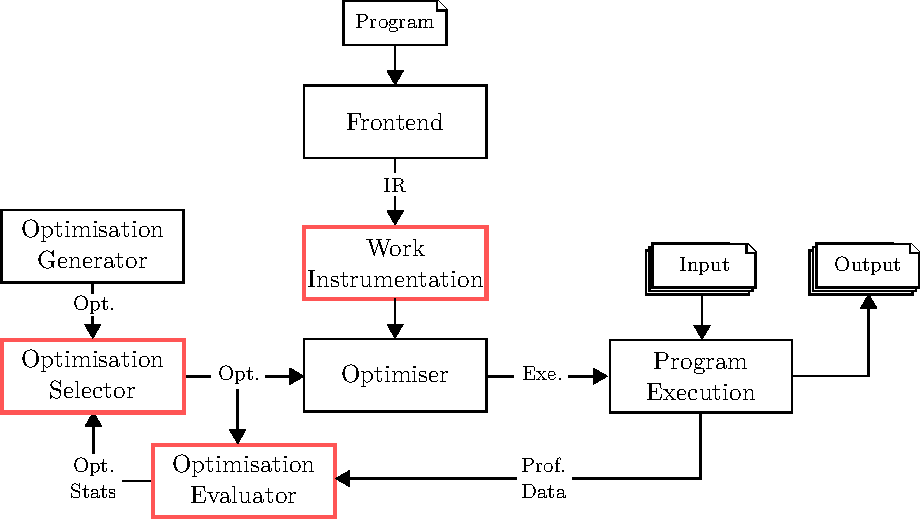
\includegraphics[width=\linewidth]{figs/infra-diagram}
    \caption{Overview of the execution engine for applying {\itercomp}.}
    \label{fig:infra-diagram}
\end{figure}
%\textbf{Describe the process step by step.}

Figure~\ref{fig:infra-diagram} shows an overview of the infrastructure required for applying online {\itercomp}
using WP as the metric of choice for evaluating optimisation sequences.
The online {\itercomp} follows as described bellow:
\begin{enumerate}
\item The program is pre-compiled to the LLVM bitcode format without optimisation.
\item The unoptimised program is instrumented for work profiling.
\item Execution-based optimisation search:
 \begin{enumerate}
   \item The current optimisation sequence is used for the re-compilation of the program.
   \item The program is executed with any input provided by the end-user.
         During the execution of the program, wall-clock time and the work metric are recorded by profiling instrumentation.
   \item If the recorded profiling for the current optimisation can be used to compute an average performance measurement within a small confidence interval,
         then a new optimisation sequence is generated.
         Otherwise, the same optimisation sequence is used for the next execution.
 \end{enumerate}
\end{enumerate}

In this work we focus mainly on the highlighted components.
The \textit{Work Instrumentation} phase focuses on providing a low-overhead instrumentation for profiling the work metric.
The instrumentation consists in adding a global counter to the program which is used to accumulate the amount of work computed during the program's execution, by means of the cost model of the instruction set.
A detailed description of the work instrumentation is presented in Section~\ref{chap:instr}.

Notice how the \textit{Work Instrumentation} phase is executed before performing any optimisation to the program.
It is critical so that the work profiling always measure the same amount of work for a given input, regardless of the optimisation sequence applied to the program.
Because the instrumentation is performed before optimising the program, it means that the work profiling derives the linear expression defined in Equation~\ref{eq:linear-work-expression}
based on the unoptimised program.
In other words, the basic blocks and the number of occurrences of the instruction in the basic blocks reflect the unoptimised program.
This particular sequence of compilation guarantees that the amount of work must is only input dependent, but consistent between different optimisation sequences.

%In both phases the goal is to improve the performance of the execution phase, but from different perspectives.
%\textit{(i.)} In the compilation phase we focused on providing a low-overhead instrumentation for profiling the work metric. This phase is responsible to improve performance by lowering the overhead of the work profiling.
%\textit{(ii.)} In the evaluation phase we proposed the use of the WP metric in order to enable {\itercomp} in an online scenario.
%This phase is responsible to improve performance by being able to properly assess different optimisations such that the best optimisation can be selected.
%Chapter~\ref{chap:instr} describes our work profiling strategy and Section~\ref{sec:metric} describes the work-based metric.

%\textbf{Talk about the process of keeping the same optimization for a given input-window and how the optimizations as selected based on the evaluation of these "evidences". Perhaps we could suggest using the Theory of Evidences at this point?!}

As the name suggests, the component called \textit{Optimisation Selector} is responsible for selecting which optimisation sequence to use for the next execution of the program.
It can either keep the same optimisation sequence used in the previous execution or start monitoring the performance of a new optimisation sequence.
An optimisation sequence can be kept for multiple executions of the program in order to gather enough measurement to compute an average performance with small statistical deviations, i.e., for which the confidence interval has a small range.
We call by \textit{Input-Window Size} the number of executions performed using the same optimisation sequence.

\subsection{Real Online Scenarios}

In most online scenarios, it is common for periods of peak usage and idle periods.
For example, mobile devices are usually intensely used during the day, with some idle periods usually when the battery is being re-charged~\citep{mpeis16}.
Similarly, many authors have considered peak and idle (or underutilised) periods of data centres~\ref{armbrust10}.

The proposed infrastructure is very well suited for these real online scenarios\footnote{
However, if idle time is almost non-existent, the proposed infrastructure can still be used by re-compiling the program with a different optimisation while multiple runs of the program are being executed.}.
In particular, periods of peak usage could be used to monitor multiple runs of the program using the same optimisation sequence, collecting the work profiling and measuring its execution time,
while periods of idleness or underutilisation could be leveraged to use the profiling statistics for selecting better optimisations and re-compiling the program.